\chapter{Approach}
The author in \cite{b6} proposes a step approach to carry out desynchronization attacks. Figure \ref{fig:Phases} shows the phases of a desynchronization attack or request smuggling. Before explaining each of the phases in request smuggling, we need to observe that there are four possible configurations between the systems:
\begin{itemize}
	\item \textbf{CL.CL : } Both the frontend and backend servers use \textsc{Content-Length} header. As we have already seen, this configuration doesn't help in realizing attacks on practical modern systems. 
	\item \textbf{CL.TE : } Frontend server uses \textsc{Content-Length} header field and Backend server uses \textsc{Transfer-Encoding} header field. 
	\item \textbf{TE.CL : } Frontend server uses \textsc{Transfer-Encoding} header field and Backend server uses \textsc{Content-Length} header field.
	\item \textbf{TE.TE : } Both the frontend and backend servers use \textsc{Transfer-Encoding} header field.
\end{itemize}
\begin{figure}
	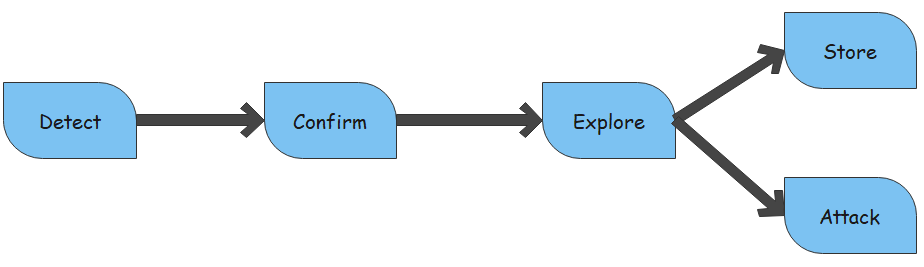
\includegraphics[width=14cm]{images/Phases}
	\caption{Phases of request smuggling}
	\label{fig:Phases}
\end{figure}
We will now look at each of the phases in detail:
\section{Detect}
The first step is to detect when a server will be vulnerable to desynchronization. A simple method here is to send a request with malicious data and poison the backend. Subsequent back to back requests are then sent to the same backend server. If the subsequent requests get an unexpected or erroneous response, we can assume that the response was due to the malicious prefix sent with the first request.  \\
However this technique isn't as simple as it looks and has a major drawback. When we try to detect desynchronization vulnerabilities in a website with a live traffic, there are numerous requests coming from many different users. If there is a normal user's request between our first malicious request and the subsequent follow up requests we send, it causes an error to the normal user and doesn't affect the follow up requests. Hence we cannot detect the vulnerability as we will not be able to observe the responses. \\
To tackle this problem, the author in \cite{b6} proposes an approach which uses server time-outs to the attacker's advantage. The configuration \textbf{CL.CL} and \textbf{TE.TE} cannot be used here for our advantage. However, \textbf{CL.TE} and \textbf{TE.CL} can be used. \\

\begin{figure}
	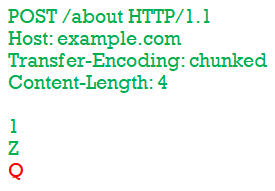
\includegraphics{images/CL.TE}
	\caption{CL.TE}
	\label{fig:CL.TE}
\end{figure}

\begin{figure}
	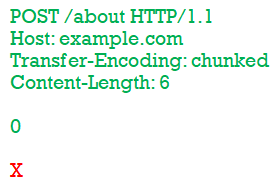
\includegraphics{images/TE.CL}
	\caption{TE.CL}
	\label{fig:TE.CL}
\end{figure}

\subsection{Case Study for \textit{Detect} phase}
Consider the example for \textbf{CL.TE} in figure \ref{fig:CL.TE}(Referenced from \cite{b6}). As \textcolor{myred}{Q} is not a valid chunk size, the frontend will forward only the information highlighted in \textcolor{mygreen}{green} and the backend will timeout waiting for next valid chunk size. \\
Consider another example for \textbf{TE.CL} in figure \ref{fig:TE.CL}(Referenced from \cite{b6}). In this request, \textcolor{mygreen}{0} is explicitly placed to force the server into considering it as the \textit{terminating chunk}. As a result, the server will timeout waiting for \textcolor{myred}{X}.\\
These observable delays are sufficient to infer that the system has a vulnerability for request smuggling.\\

\section{Confirm}
Once we are sure that a system is vulnerable for request smuggling, we need to confirm the same with the help of responses that serve as visible proofs. The technique to get such confirmation is by poisoning the backend socket. One the follow-up requests we send will fall victim to the earlier poisoning and will return a response to visibly prove that the vulnerability is present. One hindrance here is disconnection. If the first request causes an error, the backend system may have been designed to drop the connection and associated buffers. Such a disconnection will fail the attack. This can be avoided by targeting backend server endpoints which accept POST requests. 
\subsection{Case Study for \textit{Confirm} phase}
\textit{Referenced from \cite{b6}}
If the target request looks as below:

\section{Explore}
\subsection{Case Study for \textit{Confirm} phase}
\section{Store}
\subsection{Case Study for \textit{Confirm} phase}
\section{Attack}
\subsection{Case Study for \textit{Confirm} phase}